\chapter{Introduction}

\label{Chapter1_introduction} 

\begin{comment}
-------------------------------------------------
%								Chapter layout
1. Introduction
	a. Motivation
	b. Goals 
	c. Static Hand Gestures 
-------------------------------------------------
\end{comment}
%Computer science as a field is growing rapidly and expanding into many other disciplines including health care. This project is about very 
%short one paragraph or show explanation. maybe write abstract first. 

%------------------------------------------------
%	SECTION 1 Motivation
%------------------------------------------------
\section{Motivation}
Apraxia comes from the prefix “a” meaning “without” and the  Greek root word “praxis” which means “action”. Apraxia is a neurological condition that is sometimes caused by the effects of a stroke. It is a condition in which the patient is unable to exercise motor control over some of their muscles. The muscles themselves are not paralyzed or damaged, what causes these disorders are neurological conditions. In the department of Experimental Psychology researchers are studying patients with post-stroke loss of motor skills including possible cases of apraxia. The diagnosis of such a condition involves researchers presenting their patients with different movement based tests and evaluating the ease and effectiveness with which the patients are able to complete these screenings.  
	
%------------------------------------------------
%	SECTION 2 Goals
%------------------------------------------------
\section{Goals}
%what were the goals of this project and application. 

provide a application that clinicians can use to collect hand gesture data from patients. 
this data should be able to be scored by algorithms to determine how close their attempts are.
there will be two main functions of comparison that will be developed. 
the data collected should be able to be viewed inside the application
the data should be editable from within the app.
stored and retrieved from. 
the data should be saved to csv and outside data should be able to be loaded into the app by csv(as long as hand data is there)
the application should be easy for the users. it should not require a set position of their hand or wrist. 
the gestures shown should be rotateable. to allow from viewing from different angles. 



%------------------------------------------------
%	SECTION 3 Static Hand Gestures 
%------------------------------------------------
\section{Static Hand Gestures}
The gestures this project will be concerned with are ten gestures for the left hand and ten gestures for the right hand. These specific gestures were provided by clinicians during the first meeting with them to discuss the scope of the project. Below are some pictures showing what the target gestures that the users will have to imitate will look like in application. The gestures shown are are the ten gestures for the left hand, along with a rotated version of the same gestures to provide a different perspective into the shape of the gesture. The right hand gestures will be mirror images of the ones shown below. 
%Gesture1Left
\begin{figure}[H]
    \centering
    \begin{minipage}{0.5\textwidth}
        \centering
        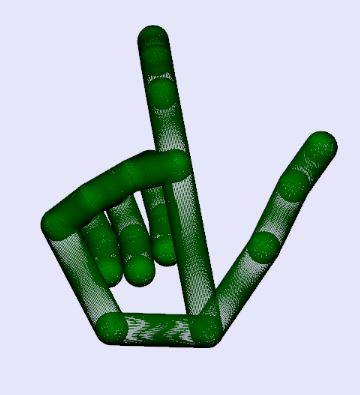
\includegraphics[scale=.75]{Figures/gesture1Left.JPG} 
        \caption[Gesture1Left]{Gesture1Left}
		\label{fig:Gesture1Left}
    \end{minipage}\hfill
    \begin{minipage}{0.5\textwidth}
        \centering
        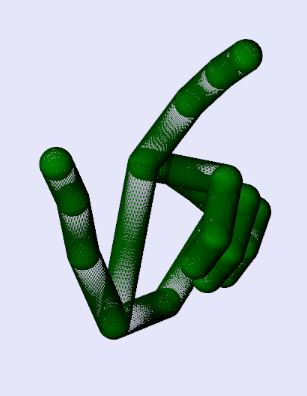
\includegraphics[scale=.7]{Figures/gesture1Left_rotated.JPG}
        \caption[Gesture1Left Rotated]{Gesture1Left rotated.}
        \label{fig:Gesture1Left_rotated}
    \end{minipage}
\end{figure}

%Gesture2Left
\begin{figure}[H]
    \centering
    \begin{minipage}{0.5\textwidth}
        \centering
        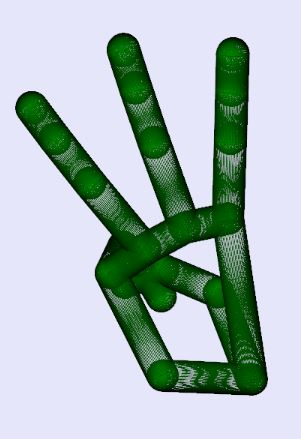
\includegraphics[scale=.75]{Figures/gesture2Left.JPG} 
        \caption[Gesture2Left]{Gesture2Left}
		\label{fig:Gesture2Left}
    \end{minipage}\hfill
    \begin{minipage}{0.5\textwidth}
        \centering
        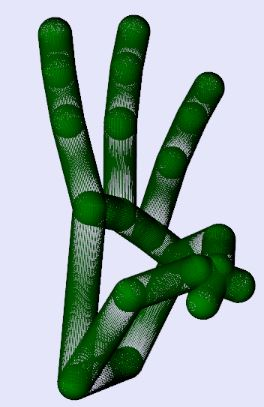
\includegraphics[scale=.75]{Figures/gesture2Left_rotated.JPG}
        \caption[Gesture2Left Rotated]{Gesture2Left rotated.}
        \label{fig:Gesture2Left_rotated}
    \end{minipage}
\end{figure}

%Gesture3Left
\begin{figure}[H]
    \centering
    \begin{minipage}{0.5\textwidth}
        \centering
        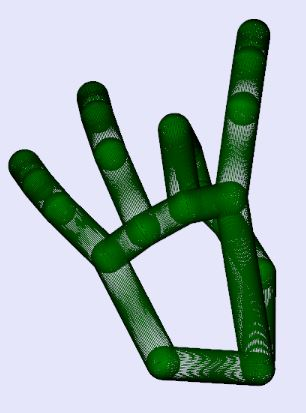
\includegraphics[scale=.75]{Figures/gesture3Left.JPG} 
        \caption[Gesture3Left]{Gesture3Left}
		\label{fig:Gesture3Left}
    \end{minipage}\hfill
    \begin{minipage}{0.5\textwidth}
        \centering
        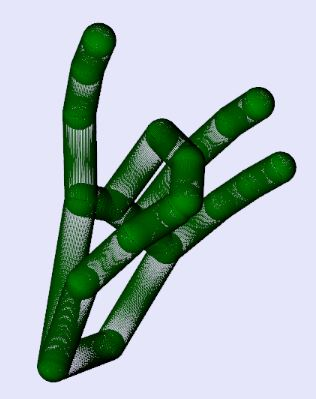
\includegraphics[scale=.75]{Figures/gesture3Left_rotated.JPG}
        \caption[Gesture3Left Rotated]{Gesture3Left rotated.}
        \label{fig:Gesture3Left_rotated}
    \end{minipage}
\end{figure}

%Gesture4Left
\begin{figure}[H]
    \centering
    \begin{minipage}{0.5\textwidth}
        \centering
        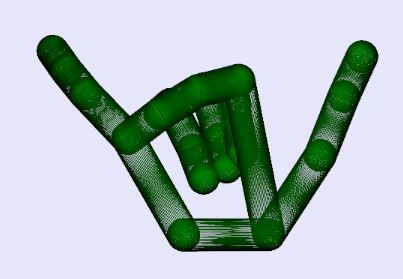
\includegraphics[scale=.75]{Figures/gesture4Left.JPG} 
        \caption[Gesture4Left]{Gesture4Left}
		\label{fig:Gesture4Left}
    \end{minipage}\hfill
    \begin{minipage}{0.5\textwidth}
        \centering
        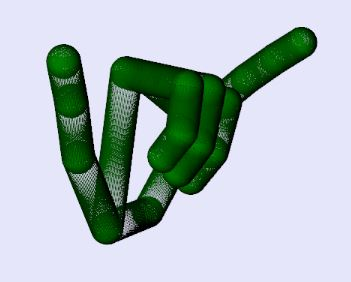
\includegraphics[scale=.75]{Figures/gesture4Left_rotated.JPG}
        \caption[Gesture4Left Rotated]{Gesture4Left rotated.}
        \label{fig:Gesture4Left_rotated}
    \end{minipage}
\end{figure}

%Gesture5Left
\begin{figure}[H]
    \centering
    \begin{minipage}{0.5\textwidth}
        \centering
        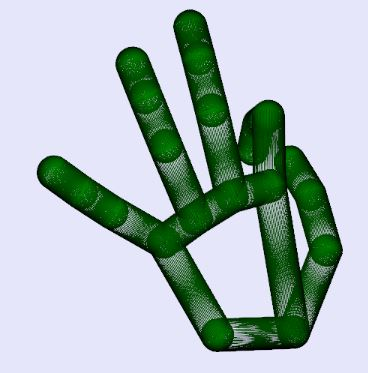
\includegraphics[scale=.75]{Figures/gesture5Left.JPG} 
        \caption[Gesture5Left]{Gesture5Left}
		\label{fig:Gesture5Left}
    \end{minipage}\hfill
    \begin{minipage}{0.5\textwidth}
        \centering
        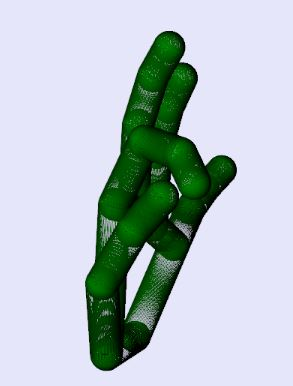
\includegraphics[scale=.75]{Figures/gesture5Left_rotated.JPG}
        \caption[Gesture5Left Rotated]{Gesture5Left rotated.}
        \label{fig:Gesture5Left_rotated}
    \end{minipage}
\end{figure}

%Gesture6Left
\begin{figure}[H]
    \centering
    \begin{minipage}{0.5\textwidth}
        \centering
        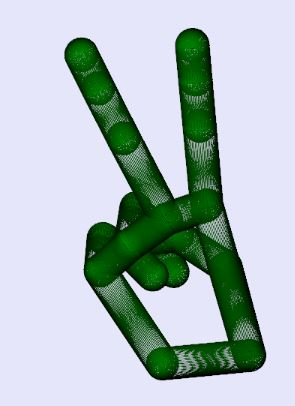
\includegraphics[scale=.75]{Figures/gesture6Left.JPG} 
        \caption[Gesture6Left]{Gesture6Left}
		\label{fig:Gesture6Left}
    \end{minipage}\hfill
    \begin{minipage}{0.5\textwidth}
        \centering
        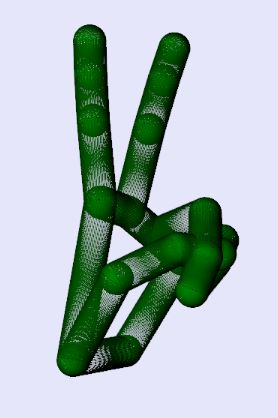
\includegraphics[scale=.7]{Figures/gesture6Left_rotated.JPG}
        \caption[Gesture6Left Rotated]{Gesture6Left rotated.}
        \label{fig:Gesture6Left_rotated}
    \end{minipage}
\end{figure}

%Gesture7Left
\begin{figure}[H]
    \centering
    \begin{minipage}{0.5\textwidth}
        \centering
        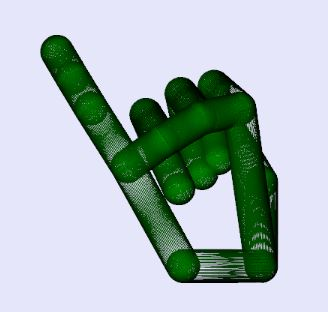
\includegraphics[scale=.75]{Figures/gesture7Left.JPG} 
        \caption[Gesture7Left]{Gesture7Left}
		\label{fig:Gesture7Left}
    \end{minipage}\hfill
    \begin{minipage}{0.5\textwidth}
        \centering
        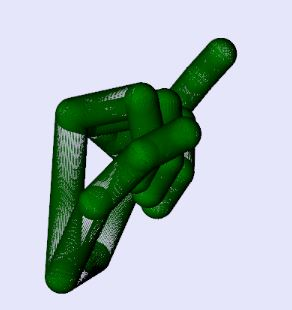
\includegraphics[scale=.75]{Figures/gesture7Left_rotated.JPG}
        \caption[Gesture7Left Rotated]{Gesture7Left rotated.}
        \label{fig:Gesture7Left_rotated}
    \end{minipage}
\end{figure}

%Gesture8Left
\begin{figure}[H]
    \centering
    \begin{minipage}{0.5\textwidth}
        \centering
        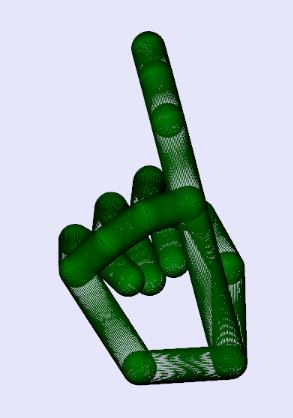
\includegraphics[scale=.75]{Figures/gesture8Left.JPG} 
        \caption[Gesture8Left]{Gesture8Left}
		\label{fig:Gesture8Left}
    \end{minipage}\hfill
    \begin{minipage}{0.5\textwidth}
        \centering
        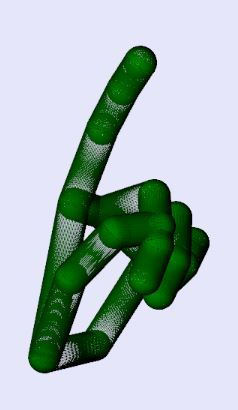
\includegraphics[scale=.75]{Figures/gesture8Left_rotated.JPG}
        \caption[Gesture8Left Rotated]{Gesture8Left rotated.}
        \label{fig:Gesture8Left_rotated}
    \end{minipage}
\end{figure}

%Gesture9Left
\begin{figure}[H]
    \centering
    \begin{minipage}{0.5\textwidth}
        \centering
        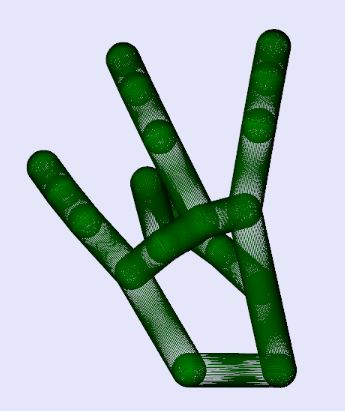
\includegraphics[scale=.75]{Figures/gesture9Left.JPG} 
        \caption[Gesture9Left]{Gesture9Left}
		\label{fig:Gesture9Left}
    \end{minipage}\hfill
    \begin{minipage}{0.5\textwidth}
        \centering
        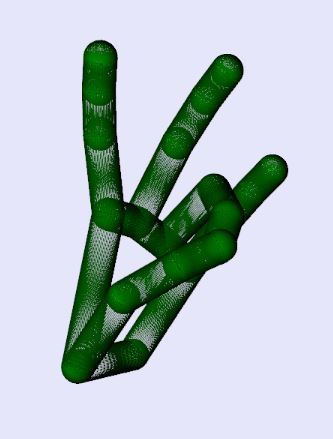
\includegraphics[scale=.75]{Figures/gesture9Left_rotated.JPG}
        \caption[Gesture9Left Rotated]{Gesture9Left rotated.}
        \label{fig:Gesture9Left_rotated}
    \end{minipage}
\end{figure}

%Gesture10Left
\begin{figure}[H]
    \centering
    \begin{minipage}{0.5\textwidth}
        \centering
        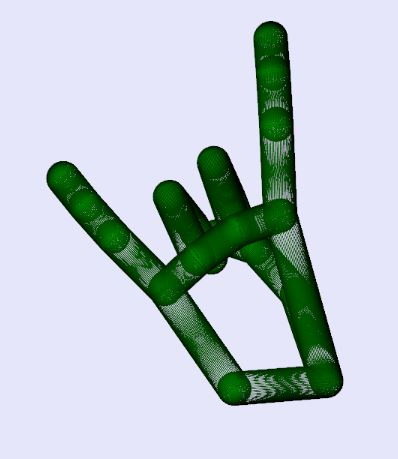
\includegraphics[scale=.75]{Figures/gesture10Left.JPG} 
        \caption[Gesture10Left]{Gesture10Left}
		\label{fig:Gesture10Left}
    \end{minipage}\hfill
    \begin{minipage}{0.5\textwidth}
        \centering
        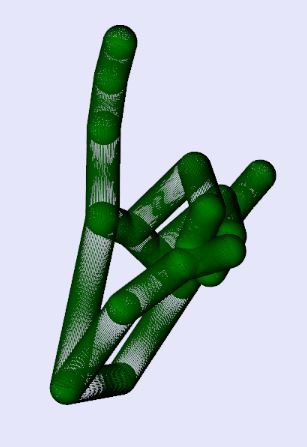
\includegraphics[scale=.75]{Figures/gesture10Left_rotated.JPG}
        \caption[Gesture10Left Rotated]{Gesture10Left rotated.}
        \label{fig:Gesture10Left_rotated}
    \end{minipage}
\end{figure}
